\subsection{Тригонометрический ряд Фурье. Теорема о почленном дифференцировании ряда Фурье. Теорема о связи гладкости функции и скорости убывания ее коэффициентов Фурье. Теорема о связи гладкости функции и скорости сходимости ее ряда Фурье. Теорема о полноте тригонометрической системы.}

\subsubsection{Теорема о почленном дифференцировании ряда Фурье.}
\begin{theorem*} Если непрерывная функция $f \in C(\left[ -\pi; \pi \right], \mathbb{C})$, принимающая на концах отрезка $\left[ -\pi; \pi \right]$ равные значения, т.е. $f(\pi) = f(-\pi)$, кусочно непрерывно дифференцируема на $\left[ -\pi; \pi \right]$, то ряд Фурье ее производной $f' \sim \sum_{-\infty}^{\infty} c_n(f') \cdot e^{inx}$ может быть получен формальным дифференцированием ряда Фурье самой функции $f \sim \sum_{-\infty}^{\infty} c_n(f) \cdot e^{inx}$, то есть получаем  $c_n(f') = inc_n(f),\, n \in \mathbb{Z}$.
\end{theorem*}
\begin{proof} Из определения коэффициентов Фурье (\ref{subsubsec:label1}) интегрированием по частям находим \begin{align*}
		c_n(f') = \dfrac{1}{2\pi}\int_{-\pi}^{\pi} f'(x)e^{-inx}\, dx = \dfrac{1}{2\pi} f(x)e^{-inx}\biggl|_{-\pi}^{\pi} + \dfrac{in}{2\pi}\int_{-\pi}^{\pi} f(x)e^{-inx}\, dx = inc_n(f) \text{, т.к. } f(\pi)e^{-in\pi} - f(-\pi)e^{in\pi} = 0.
	\end{align*}
\end{proof}

\subsubsection{Теорема о связи гладкости функции и скорости убывания ее коэффициентов Фурье.}
\begin{theorem*} Пусть $f(x): \left[-\pi; \pi\right] \to \mathbb{C}$ такова, что
	\begin{itemize}
		\item[1)] функция $(m-1)$ раз непрерывно дифференцируема на $\left[ -\pi; \pi \right]$, $m \in \mathbb{N}$,
		\item[2)] $f^{(k)}(-\pi) = f^{(k)}(\pi)$ при всех $k = 0,1, \dotsc, (m-1)$,
		\item[3)] функция $(m)$ раз кусочно--непрерывно дифференцируема (другими словами: $f(x)\text{ имеет на } \left[ -\pi; \pi \right]$ кусочно непрерывную производную $f^{(m)}$ порядка $m$),
	\end{itemize}
	тогда $c_n(f^{(m)}) = (in)^m \cdot c_n(f),\, n \in \mathbb{Z}$ и $\left|c_n(f)\right| = \dfrac{\gamma_n}{|n|^m} = o\left(\dfrac{1}{n^m}\right)$ , причем $\gamma_n = |c_n(f^{(m)})|$ и ряд $\sum_{-\infty}^{\infty} \gamma_n^2$ сходится при  $n \to \infty, n \in \mathbb{Z}$.
\end{theorem*}
\begin{proof} Первое соотношение получается в результате $m$--кратного использования равенства $c_n(f') = inc_n(f)$ (из пункта выше): $c_n(f^{(m)}) = (in) \cdot c_n(f^{(m-1)}) = \dotsc  = (in)^mc_n(f)$. 
	
	Второе соотношение получается с учетом неравенства Бесселя (\ref{subsubsec:label2}): $\sum_{-\infty}^{\infty} |c_n(f^{(m)})|^2 \leqslant \dfrac{1}{2\pi} \int_{-\pi}^{\pi}|f^{(m)}|^2(x)\, dx$ -- это число $\implies \gamma_n = |c_n(f^{(m)})| \to 0$, и ряд $\sum_{-\infty}^{\infty} |c_n(f^{(m)})|^2 = \sum_{-\infty}^{\infty} \gamma_n^2 $ сходится.  Следовательно,  $c_n(f) = o\left(\dfrac{1}{n^m}\right)$.
	
\end{proof}
\subsubsection{Теорема о связи гладкости функции и скорости сходимости ее ряда Фурье.}
\begin{theorem*} Если $f(x): \left[-\pi; \pi\right] \to \mathbb{C}$ такова, что
	\begin{itemize}
		\item[1)] функция $(m-1)$ раз непрерывно дифференцируема на $\left[ -\pi; \pi \right]$, $m \in \mathbb{N}$,
		\item[2)] $f^{(k)}(-\pi) = f^{(k)}(\pi)$ при всех $k = 0,1, \dotsc, (m-1)$,
		\item[3)] функция $(m)$ раз кусочно--непрерывно дифференцируема (другими словами: $f(x)\text{ имеет на } \left[ -\pi; \pi \right]$ кусочно непрерывную производную $f^{(m)}$ порядка $m \geqslant 1$),
	\end{itemize}
	то ряд Фурье функции $f$ сходится к $f$ абсолютно и равномерно на отрезке $\left[-\pi; \pi\right]$, причем отклонение $n$--й частичной суммы $S_n(x)$ ряда Фурье от $f(x)$ на всем отрезке $\left[-\pi; \pi\right]$ имеет оценку $|f(x) - S_n(x)| \leqslant \dfrac{\varepsilon_n}{n^{m - 1/2}}$, где ${\varepsilon_n}$ -- стремящаяся к нулю последовательность положительных чисел при $n \to \infty$.
\end{theorem*} 
\begin{proof} Частичную сумму ряда Фурье(\ref{subsubsec:label3}) запишем в компактной форме: $S_n(x) = \sum_{-n}^{n} c_k(f)e^{ikx}$.
	
	В соответствии с условиями на функцию $f$ и по теореме о связи гладкости функции и скорости убывания ее коэффициентов Фурье имеем:
	$\left|c_k(f)\right| = \dfrac{\gamma_k}{|k|^m}$, причем $\sum \dfrac{\gamma_k}{|k|^m} < \infty$ (поскольку $0 \leqslant \dfrac{\gamma_k}{|k|^m} \leqslant \dfrac12 \left(\gamma_k^2 + \dfrac{1}{k^{2m}}\right)$ по неравенству о среднем и  $m \geqslant 1$, имеем $\sum \dfrac{\gamma_k}{|k|^m} < \infty$). Значит, последовательность $S_n(x)$ на  отрезке $\left[ -\pi; \pi \right]$ равномерно сходится по мажорантному признаку Вейерштрасса для рядов (или критерию Коши для последовательностей).
	
	В силу достаточного условия сходимости ряда Фурье в точке предел $S(x)$ последовательности $S_n(x)$ совпадает с $f(x)$, поскольку функция $f$ удовлетворяет условиям Дини в каждой точке отрезка $\left[ -\pi; \pi \right]$ и т.к.  	$f(-\pi) = f(\pi)$	, то функция $f$ периодически продолжается на $\mathbb{R}$ с сохранением условий Дини в любой точке $x \in \mathbb{R}$.
	
	Переходим к оценке. Используем последнее равенство из конца формулировки теоремы 11.2:
	\begin{align*}
		|f(x) - S_n(x)| = |S(x) - S_n(x)| = \left|\sum_{\pm k = n + 1}^{\infty} c_k(f)e^{ikx} \right| &\leqslant \sum_{\pm k = n + 1}^{\infty} |c_k(f)| =  \sum_{\pm k = n + 1}^{\infty} \dfrac{\gamma_k}{|k|^m} \leqslant \\
		&\leqslant \left( \sum_{\pm k = n + 1}^{\infty} \gamma_k^2\right)^{1/2} \left( \sum_{\pm k = n + 1}^{\infty} 1/k^{2m}\right)^{1/2}
	\end{align*}	
	Первый множитель в правой части неравенства Коши--Буняковского стремится к нулю при $n \to \infty$, т.к. $\sum_{-\infty}^{\infty} \gamma_k^2 < \infty$. 
	
	Далее (см. рис.104) оценка:
	\begin{align*}
		\sum_{k = n + 1}^{\infty} \dfrac{1}{k^{2m}} \leqslant \int_{n}^{\infty} \dfrac{dx}{x^{2m}} = \dfrac{1}{2m-1} \cdot \dfrac{1}{n^{2m-1}}.
	\end{align*}
	\begin{center}
		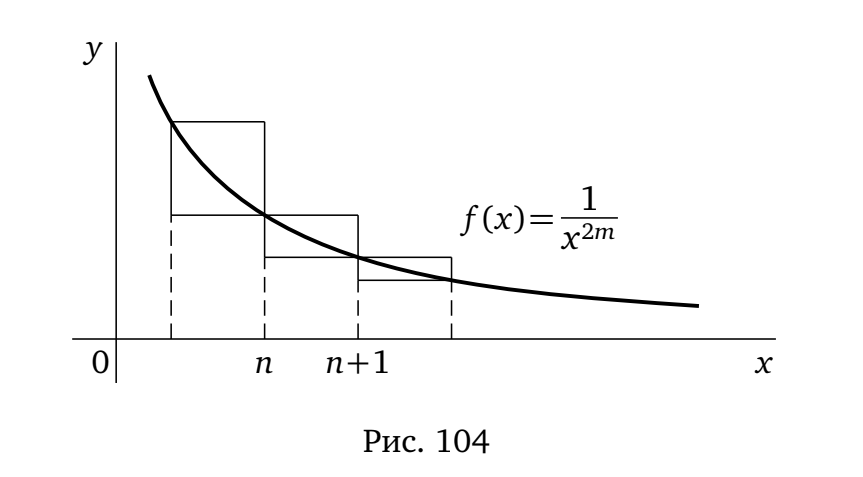
\includegraphics[scale=0.5]{img/pic104.png}
	\end{center}
	Таким образом, получается то, что и утверждает теорема.
\end{proof}

\subsubsection{Теорема о полноте тригонометрической системы.}

\begin{theorem*} \ Любая функция $f \in \mathcal{R}_2(\left[ -\pi; \pi \right], \mathbb{R})$ (т.е. $f$ интегрируема на любом отрезке $\left[a; b\right] \subset \left( -\pi; \pi \right)$ и $f^2(x)$ интегрируема хотя бы в несобственном смысле на отрезке $\left[ -\pi; \pi \right]$) может быть сколь угодно точно приближена (по--научному: апроксимирована) в средне--квадратичном тригонометрическими многочленами.
\end{theorem*}
\begin{proof} Любую функцию $f \in \mathcal{R}_2$  можно сколь угодно точно  приблизить финитной функцией $g \in \mathcal{R}_2$ на $\left[-\pi; \pi\right]$, интегрируемой по Риману на этом отрезке (функция $g$ называется \textit{финитной} на $[-\pi; \pi]$, если существует $[a; b]\subset(-\pi; \pi)$ и $g = 0$ при $x \in [-\pi; \pi] \backslash [a; b]$). Функцию $g$ мы приближаем кусочно постоянной функцией $h$ на отрезке $[-\pi; \pi]$.   Функцию $h$ приближаем ломанной функцией $l$, которая на концах отрезка будет равна нулю. Тогда ломанная $l$ -- это кусочно непрерывная дифференцируема функция, и она сколь угодно точно приближается тригонометрическим многочленом.  Из всего этого получаем, что любая функция $f \in \mathcal{R}_2$  по норме пространства $\mathcal{R}_2$  сколь угодно точно приближается  тригонометрическим многочленом.
\end{proof}